\documentclass{article}

% Language setting
% Replace `english' with e.g. `spanish' to change the document language
\usepackage[english]{babel}

% Set page size and margins
% Replace `letterpaper' with `a4paper' for UK/EU standard size
\usepackage[letterpaper,top=2cm,bottom=2cm,left=3cm,right=3cm,marginparwidth=1.75cm]{geometry}
% Useful packages
\usepackage{multicol}
\usepackage{amsmath}
\usepackage{amssymb}
\usepackage{graphicx}
\usepackage[framemethod=tikz]{mdframed}
\usepackage{array}
\usepackage{blindtext}
%\usepackage[paperwidth=10cm]{geometry}
\usepackage{tkz-euclide}
%\usepackage{tikz}
\usetikzlibrary{
  circuits.logic,
  circuits.logic.US,
  positioning
}

\usepackage[colorlinks=true, allcolors=blue]{hyperref}

\title{Line Assignment}
\author{Anusha Jella}
\begin{document}
\maketitle
\begin{multicols}{2}
\paragraph{\textbf{Problem: } \textbf{In Fig.1, PQRS and ABRS are parallelograms
and X is any point on side BR. Show that  }}
\begin{enumerate}
    \item \textbf{ar (PQRS) = ar(ABRS)}
    \item \textbf{ar(AXS) = 1/2 ar(PQRS)}
\end{enumerate}
%\begin{figure}[h]
\centering
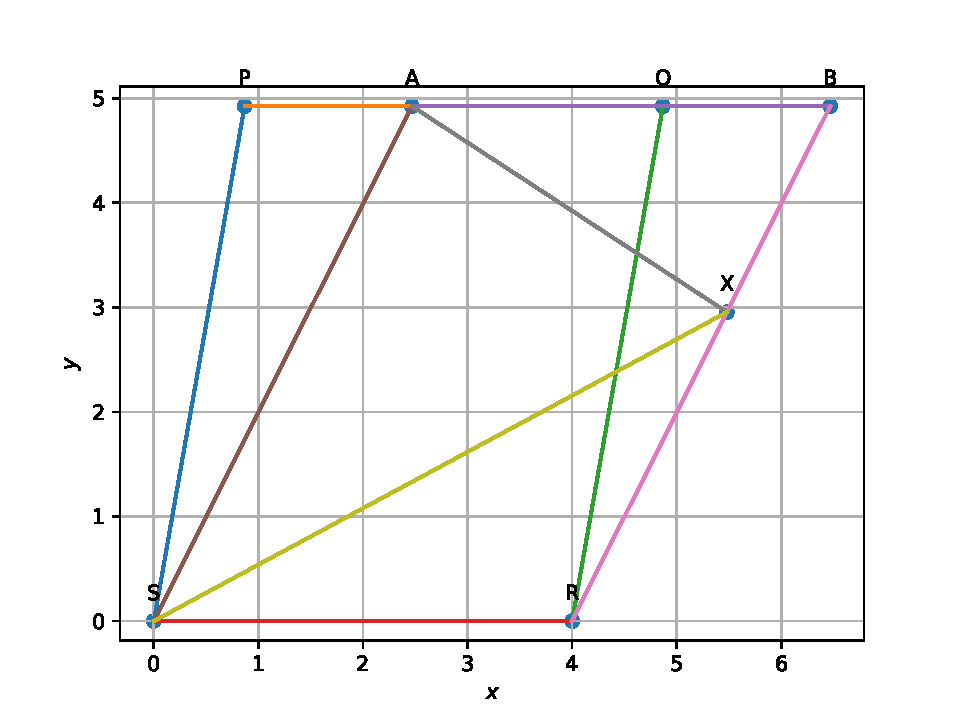
\includegraphics[width=\columnwidth]{parallelogram1.pdf} 
\centering{Fig 1. Parallelogram}
\label{fig:triangle}
%\end{figure}

\section*{\textbf{Solution 1:}}
\begin{flushleft}
Two parallelograms PQRS and ABRS, on the same base SR and between the same parallels PB and SR are given (see Fig.1).\\
We need to prove that ar(PQRS) = ar(ABRS).\\
Let, In PQRS 
\end{flushleft}
\begin{align}
           \boldsymbol{S}-\boldsymbol{R}&=\boldsymbol{p1}\hfill \\
           \boldsymbol{S}-\boldsymbol{P}&=\boldsymbol{p2}\hfill \\
           \boldsymbol{P}-\boldsymbol{Q} &=\boldsymbol{q1}\hfill \\
           \boldsymbol{R}-\boldsymbol{Q}&=\boldsymbol{q2}
\end{align}
 According to parrallelogram condition \\
\begin{align}
\lVert{\textbf{p1}}\rVert =\lVert{\textbf{q1}}\rVert \&\& \lVert{\textbf{p2}}\rVert =\lVert{\textbf{q2}}\rVert
\end{align}
\hspace{-4cm}Let,In ABRS
\begin{align}
           \boldsymbol{S}-\boldsymbol{R}&=\boldsymbol{s1} \hfill \\
           \boldsymbol{S}-\boldsymbol{A}&=\boldsymbol{s2} \hfill \\
           \boldsymbol{A}-\boldsymbol{B}&=\boldsymbol{r1} \hfill \\
           \boldsymbol{R}-\boldsymbol{B}&=\boldsymbol{r2}
\end{align} 
\hspace{-1cm}According to parallelogram condition 
\begin{align}
\lVert{\textbf{s1}}\rVert &=\lVert{\textbf{r1}}\rVert \&\& \lVert{\textbf{s2}}\rVert =\lVert{\textbf{r2}}\rVert
\end{align}
\hspace{-2cm}Area of parallelogram PQRS
\begin{align}
\boldsymbol{p1} X \boldsymbol{p2}       
\end{align}        
\hspace{-1cm}Now, area of parallelogram ABRS
\begin{align}
&=\boldsymbol{SR} X \boldsymbol{SA}
\end{align}
\begin{align}
&=\boldsymbol{s1} X \boldsymbol{s2}
\end{align}
\begin{align}
&=\boldsymbol{SR} X \boldsymbol{(SP+PA)}
\end{align}
 \hspace{3cm} [$\boldsymbol{PA}$ $\parallel$ $\boldsymbol{PQ}$ $\therefore$ $\boldsymbol{PA}$ =k $\boldsymbol{p1}$]
\begin{align}
 &=\boldsymbol{p1} X (\boldsymbol{p2}+k \boldsymbol{p1})
\end{align}  
[from [5] and [10] $\lVert{\textbf{p1}}\rVert$ =$\lVert{\textbf{s1}}\rVert$] 
\begin{align}
&=\boldsymbol{p1} X \boldsymbol{p2} +\boldsymbol{p1} X k \boldsymbol{p1}
\end{align}
\begin{align}
&=\boldsymbol{p1} X \textbf{p2} +k(\boldsymbol{p1} X \boldsymbol{p1})
\end{align}
\begin{align}
&=\boldsymbol{p1} X \boldsymbol{p2}
\end{align}     
   \hspace{3cm} [$\therefore$ $\boldsymbol{p1}$ X $\boldsymbol{p1}$ =0]\\
=Area of parallelogram ABRS\\
\begin{enumerate}
\item[] Hence proved
\item[] So, from [11] and [18] PQRS and ABRS parallalograms are equal in area.
\end{enumerate} 
\section*{solution 2:}
\begin{flushleft}
Let $\Delta{AXS}$ and parallelogram ABRS be on the same base AS and between the same parallels $\boldsymbol{AS}$ and $\boldsymbol{BR}$ (see Fig. 1).\\
You wish to prove that
\end{flushleft}
ar (AXS) = $\frac{1}{2}$ ar (PQRS)\\
\begin{flushleft}
Draw BY $\parallel$ AS to obtain another parallelogram AXYS as in Fig 2. Now parallelograms ABRS and AXYS are on the same base AS and between the same parallels AS and BY.
\end{flushleft}
\begin{align}
\therefore ar (ABRS) = ar (AXYS) \text{(By Solution 1)}
\end{align}
\begin{flushleft}
But $\Delta{AXS}$ $\cong$ $\Delta{XYS}$ (Diagonal SX divides parallelogram AXYS into two congruent triangles.)
\end{flushleft}
\begin{align}
           \boldsymbol{A}-\boldsymbol{X}&=\boldsymbol{a1} \hfill \\
           \boldsymbol{S}-\boldsymbol{X}&=\boldsymbol{d1}  \hfill \\
           \boldsymbol{X}-\boldsymbol{Y}&=\boldsymbol{x1}  \hfill \\
           \boldsymbol{Y}-\boldsymbol{S}&=\boldsymbol{x2} \hfill\\
           \boldsymbol{S}-\boldsymbol{A}&=\boldsymbol{x3} 
\end{align}           
\hspace{-2cm}from parallelogram condition 
\begin{align}
\boldsymbol{a1}=\boldsymbol{x2} \&\&  \boldsymbol{x3}=\boldsymbol{x1}
\end{align}
\begin{align}
ar (AXS) = ar (SXY)
\end{align}
\hspace{-2cm}Therefore,
\begin{enumerate}
\item[]ar (AXYS) =ar (AXS) +ar (XYS)
\item[]ar (AXS)=$\frac{1}{2}$ * ($\boldsymbol{x3}$ X $\boldsymbol{a1}$)
\item[]ar (AXYS)=($\boldsymbol{x3}$  X $\boldsymbol{a1}$) $\implies$ $\boldsymbol{SA}$ X$\boldsymbol{AX}$ 
\item[]ar (AXS)=1/2 ar (AXYS)\\
    \hspace{1.5cm}    =$\frac{1}{2}$($\boldsymbol{SA}$ X$\boldsymbol{AX}$)\\
    \hspace{1.5cm}    =$\frac{1}{2}$ ($\boldsymbol{SA}$ X $\boldsymbol{(AB+BX)}$)\\
    \hspace{1.5cm}    =$\frac{1}{2}$ (($\boldsymbol{s2}$ + k $\boldsymbol{s1}$) X ($\boldsymbol{s1}$+ k1($\boldsymbol{s2}$ + k$\boldsymbol{s1}$)))
\item[[] =$\frac{1}{2}$ ($\boldsymbol{s1}$ X $\boldsymbol{s2}$)           [ $\boldsymbol{a}$ X $\boldsymbol{a}$ =0] \\
       =$\frac{1}{2}$ ($\boldsymbol{SR}$ X$\boldsymbol{SA}$)     
\end{enumerate}
\begin{flushleft}
This gives ar (AXS) = $\frac{1}{2}$ ar (ABRS) [From (1) and (3)]\\
           ar (AXS) = $\frac{1}{2}$ ar (PQRS) [From solution 1] \\
\end{flushleft}
 \section*{Construction}
 \begin{flushleft}
 The following python code is used for constructing PQRS and ABRS parallalograms.
 \end{flushleft}
 \begin{mdframed}
   \url{https://github.com/AnushaJella/assigment_line/blob/main/code/asgn1.py}\\
\end{mdframed}
See Fig 1 for the input parameters in Table 1.\\
{\setlength\extrarowheight{2pt}
\begin{tabular}{|c|c|c|}
	\hline
	\textbf{Symbol}&\textbf{Value}&\textbf{Description}\\
	\hline
	S&$\begin{pmatrix}
	0\\0\\
	\end{pmatrix} $&S Point\\
	\hline
	a&4& SR\\
	\hline
	$\theta$&80$^{\circ}$&$\angle$RSP\\
	\hline
	b & 5 & SP\\
	\hline
	k& 1.5 &Point A\\
	\hline
\end{tabular}
}\\
\centering {Table 1}\\
\begin{flushleft}
For construction, let $\boldsymbol{S}=0$, $\boldsymbol{P}$,$\boldsymbol{R}$ are input vectors. \\
the fourth point be\\
\end{flushleft}
\centering $\boldsymbol{Q}$=$\boldsymbol{P}$+$\boldsymbol{R}$-$\boldsymbol{S}$ \\
\begin{flushleft}
choose k value and define\\
\end{flushleft}
\begin{align*}
\boldsymbol{A} =\frac{
	k \boldsymbol{P}}{k+1}
\end{align*}
\begin{flushleft}
B is fourth vertex of ABRS parallelogram\\
\end{flushleft}
\centering $\boldsymbol{B}$=$\boldsymbol{A}$+$\boldsymbol{R}$-$\boldsymbol{S}$ \\
\begin{flushleft}
X be any point on BR k value and define\\
\end{flushleft}
\begin{align*}
\boldsymbol{X} =\frac{
	k \boldsymbol{B}}{k+1}
\end{align*}
\begin{flushleft}
draw a line parallel from S such that AX $\parallel$ SY. \\
So,AXYS is a parallalogram
\end{flushleft}
\centering {$\boldsymbol{Y}$=$\boldsymbol{S}$+$\boldsymbol{X}$-$\boldsymbol{A}$} \\
%\centering {\includegraphics[scale=0.5]{rect22.pdf}}
\begin{flushleft}
\textbf{Proof:}Two parallelograms PQRS and ABRS, on
the same base SR and between the same parallels
PB and SR are given (see Fig.1).\\
We need to prove that ar (PQRS) = ar (ABRS).\\
In $\Delta$ PSA and $\Delta$ QRB,
\end{flushleft}
\begin{align}
\angle SPA = \angle RQB 
\end{align}
  \hspace{1cm}(Corresponding angles from PS $\parallel$ RQ and transversal PB) \\
\begin{align}
\angle PAS = \angle QBR
\end{align}
  \hspace{1cm} (Corresponding angles from AS $\parallel$ BR and transversal PB) \\
\begin{align}
Therefore, \angle PSA = \angle QRB
\end{align}
   \hspace{1cm} (Angle sum property of a triangle) \\
\begin{align}
Also, PS = QR
\end{align}
\hspace{0.5cm}  (Opposite sides of the parallelogram PQRS)
So, $\Delta$ PSA $\cong$ $\Delta$ QRB \\
 \hspace{0.5cm}(By ASA rule, using (27), (29), and (30))
\begin{align}
Therefore, ar (PSA) = ar (QRB) 
\end{align}
\hspace{1cm}(Congruent figures have equal areas)
\begin{enumerate}
\item[] Now, \\
\item[]ar (PQRS) = ar (PSA) + ar (AQRS)\\
\item[]= ar (QRB) + ar (AQRS) [From(33)]\\
\item[]= ar (ABRS)
\end{enumerate}
So, parallelograms PQRS and ABRS are equal in area.	  
\end{multicols}{2}
\end{document}